% Options for packages loaded elsewhere
\PassOptionsToPackage{unicode}{hyperref}
\PassOptionsToPackage{hyphens}{url}
\documentclass[
  ignorenonframetext,
]{beamer}
\newif\ifbibliography
\usepackage{pgfpages}
\setbeamertemplate{caption}[numbered]
\setbeamertemplate{caption label separator}{: }
\setbeamercolor{caption name}{fg=normal text.fg}
\beamertemplatenavigationsymbolsempty
% remove section numbering
\setbeamertemplate{part page}{
  \centering
  \begin{beamercolorbox}[sep=16pt,center]{part title}
    \usebeamerfont{part title}\insertpart\par
  \end{beamercolorbox}
}
\setbeamertemplate{section page}{
  \centering
  \begin{beamercolorbox}[sep=12pt,center]{section title}
    \usebeamerfont{section title}\insertsection\par
  \end{beamercolorbox}
}
\setbeamertemplate{subsection page}{
  \centering
  \begin{beamercolorbox}[sep=8pt,center]{subsection title}
    \usebeamerfont{subsection title}\insertsubsection\par
  \end{beamercolorbox}
}
% Prevent slide breaks in the middle of a paragraph
\widowpenalties 1 10000
\raggedbottom
\AtBeginPart{
  \frame{\partpage}
}
\AtBeginSection{
  \ifbibliography
  \else
    \frame{\sectionpage}
  \fi
}
\AtBeginSubsection{
  \frame{\subsectionpage}
}
\usepackage{iftex}
\ifPDFTeX
  \usepackage[T1]{fontenc}
  \usepackage[utf8]{inputenc}
  \usepackage{textcomp} % provide euro and other symbols
\else % if luatex or xetex
  \usepackage{unicode-math} % this also loads fontspec
  \defaultfontfeatures{Scale=MatchLowercase}
  \defaultfontfeatures[\rmfamily]{Ligatures=TeX,Scale=1}
\fi
\usepackage{lmodern}
\ifPDFTeX\else
  % xetex/luatex font selection
\fi
% Use upquote if available, for straight quotes in verbatim environments
\IfFileExists{upquote.sty}{\usepackage{upquote}}{}
\IfFileExists{microtype.sty}{% use microtype if available
  \usepackage[]{microtype}
  \UseMicrotypeSet[protrusion]{basicmath} % disable protrusion for tt fonts
}{}
\makeatletter
\@ifundefined{KOMAClassName}{% if non-KOMA class
  \IfFileExists{parskip.sty}{%
    \usepackage{parskip}
  }{% else
    \setlength{\parindent}{0pt}
    \setlength{\parskip}{6pt plus 2pt minus 1pt}}
}{% if KOMA class
  \KOMAoptions{parskip=half}}
\makeatother
\usepackage{longtable,booktabs,array}
\usepackage{caption}
\captionsetup[table]{skip=6pt}
\newcounter{none} % for unnumbered tables
\usepackage{calc} % for calculating minipage widths
\usepackage{caption}
% Make caption package work with longtable
\makeatletter
\def\fnum@table{\tablename~\thetable}
\makeatother
\usepackage{graphicx}
\makeatletter
\newsavebox\pandoc@box
\newcommand*\pandocbounded[1]{% scales image to fit in text height/width
  \sbox\pandoc@box{#1}%
  \Gscale@div\@tempa{\textheight}{\dimexpr\ht\pandoc@box+\dp\pandoc@box\relax}%
  \Gscale@div\@tempb{\linewidth}{\wd\pandoc@box}%
  \ifdim\@tempb\p@<\@tempa\p@\let\@tempa\@tempb\fi% select the smaller of both
  \ifdim\@tempa\p@<\p@\scalebox{\@tempa}{\usebox\pandoc@box}%
  \else\usebox{\pandoc@box}%
  \fi%
}
% Set default figure placement to htbp
\def\fps@figure{htbp}
\makeatother
\setlength{\emergencystretch}{3em} % prevent overfull lines
\providecommand{\tightlist}{%
  \setlength{\itemsep}{0pt}\setlength{\parskip}{0pt}}
% Auto-generated by infrastructure/rendering/_pdf_latex_helpers.py::extract_math_font_preamble.
% Minimal header passed to Pandoc via -H so Beamer slides pick up the same math font
% as the combined-PDF path. Adjust the manuscript's preamble.md to change the font globally.
\usepackage{unicode-math}
\setmathfont{latinmodern-math.otf}

% Manuscript macro/package fallbacks (newcommand -> providecommand).
% Core mathematics
\usepackage{amsmath}
\usepackage{amssymb}
% Document layout
% Tables
\usepackage{booktabs}
% Algorithm typesetting (for pseudocode in §2 Methodology)
% Code listings
\usepackage{listings}
% Typography and formatting
% Cross-references and citations
% ── Unicode-capable mono font for code listings ──────────────────────
% JuliaMono (TeX Live 2026) covers the full math/Greek glyph set used in
% scientific code blocks; the default lmmono lacks \alpha/\mu/\partial/\nabla.
%
% The hardcoded TeX Live 2026 path below is portable to most macOS / Linux
% TeX Live installs that placed JuliaMono under the default texmf-dist path.
% If your TeX Live version differs (e.g., 2025, 2027) or your distribution
% installs fonts elsewhere, comment out the explicit Path = line — fontspec
% will then search the system font path. If JuliaMono is not installed at
% all, comment out the whole block; xelatex falls back to lmmono with
% reduced Unicode coverage but the document still compiles.
% Math font for unicode-math: Latin Modern Math (TeX Live) has full BMP
% coverage including U+2223 (\mid), U+226A/226B (\ll/\gg), and the Greek/
% blackboard letters used in equations. Without an explicit \setmathfont,
% unicode-math falls back to lmroman text font which lacks several glyphs
% and emits "Missing character" warnings on every \mid in math mode.

% Slide layout defaults for warning-clean scientific decks.
\usepackage{etoolbox}
\IfFileExists{xurl.sty}{\usepackage{xurl}}{}
\IfFileExists{seqsplit.sty}{\usepackage{seqsplit}}{\newcommand{\seqsplit}[1]{#1}}
\protected\def\breakseq#1{\seqsplit{#1}}
\protected\def\breaktt#1{\begingroup\ttfamily\seqsplit{#1}\endgroup}
\setlength{\emergencystretch}{6em}
\tolerance=5000
\hbadness=10000
\hfuzz=1pt
\setlength{\tabcolsep}{2pt}
\AtBeginEnvironment{longtable}{\tiny\renewcommand{\arraystretch}{0.86}\setlength{\tabcolsep}{1pt}}
\AtBeginEnvironment{tabular}{\tiny\renewcommand{\arraystretch}{0.86}\setlength{\tabcolsep}{1pt}}
\AtBeginEnvironment{equation}{\tiny}
\AtBeginEnvironment{equation*}{\tiny}
\AtBeginEnvironment{align}{\tiny}
\AtBeginEnvironment{align*}{\tiny}
\AtBeginEnvironment{itemize}{\footnotesize}
\AtBeginEnvironment{enumerate}{\footnotesize}
\AtBeginEnvironment{description}{\footnotesize}
\setbeamerfont{caption}{size=\tiny}
\setbeamerfont{caption name}{size=\tiny}
\setbeamerfont{normal text}{size=\small}
\setbeamerfont{frametitle}{size=\small}
\setbeamerfont{section title}{size=\footnotesize}
\setbeamerfont{subsection title}{size=\footnotesize}
\setbeamertemplate{section page}{%
  \centering
  \begin{beamercolorbox}[sep=12pt,center,wd=\paperwidth]{section title}
    \parbox{0.86\paperwidth}{\centering\usebeamerfont{section title}\insertsection\par}
  \end{beamercolorbox}
}
\setbeamertemplate{subsection page}{%
  \centering
  \begin{beamercolorbox}[sep=8pt,center,wd=\paperwidth]{subsection title}
    \parbox{0.86\paperwidth}{\centering\usebeamerfont{subsection title}\insertsubsection\par}
  \end{beamercolorbox}
}
\setlength{\abovecaptionskip}{2pt}
\setlength{\belowcaptionskip}{0pt}

% Natbib and cross-reference fallbacks — slides don't load natbib
% or cleveref, but combined-PDF manuscript prose may emit these
% commands. The fallback renders citations as a bracketed key list
% and cross-references as detokenized labels so slides don't fail on
% undefined control sequences or raw underscores. \providecommand is
% a no-op if packages load later.
\providecommand{\citep}[1]{[#1]}
\providecommand{\citet}[1]{#1}
\providecommand{\citealp}[1]{#1}
\providecommand{\citeauthor}[1]{#1}
\providecommand{\citeyear}[1]{#1}
\providecommand{\cref}[1]{\texttt{\detokenize{#1}}}
\providecommand{\Cref}[1]{\texttt{\detokenize{#1}}}
\providecommand{\crefrange}[2]{\texttt{\detokenize{#1}}--\texttt{\detokenize{#2}}}
\providecommand{\Crefrange}[2]{\texttt{\detokenize{#1}}--\texttt{\detokenize{#2}}}
\providecommand{\paragraph}[1]{\textbf{#1}\ }

\newtheorem{proposition}{Proposition}
\newtheorem{hypothesis}{Hypothesis}
\newtheorem{remark}[theorem]{Remark}
\newtheorem{axiom}{Axiom}
\newtheorem{property}{Property}
\usepackage{bookmark}
\IfFileExists{xurl.sty}{\usepackage{xurl}}{} % add URL line breaks if available
\urlstyle{same}
% fallback for those not using the hyperref driver hyperxmp:
\makeatletter
\@ifundefined{xmpquote}{\newcommand{\xmpquote}[1]{#1}}{}
\makeatother
\hypersetup{
  hidelinks,
  pdfcreator={LaTeX via pandoc}}

\author{\texorpdfstring{}{}}
\date{}

\begin{document}

\section{Securing Agent Orchestration: Mediation Points Across
Protocols}\label{sec:orchestration}

\begin{frame}[allowframebreaks]{Securing Agent Orchestration: Mediation
Points Across Protocols}
Multi-agent systems introduce a security surface that single-agent
analysis misses: the orchestration layer that decomposes tasks,
dispatches workers, aggregates results, and holds credentials on their
behalf. Compartmentalization at the operating-system layer separates
trust domains, but an orchestration layer recreates privileged
intermediaries in software above the OS. If that layer is compromised
--- or merely persuaded --- every domain it can reach is reachable at
once. This section treats orchestration as a first-class security
surface with its own trust boundaries, its own least-privilege
requirements, and its own audit obligations, extending the authority
architecture of sec.~10. Its organizing device
is a taxonomy of mediation points: the ten places where an orchestration
stack can interpose a check between an agent's capability and an agent's
action.
\end{frame}

\begin{frame}[allowframebreaks]{The orchestrator as privileged
intermediary}
\protect\phantomsection\label{the-orchestrator-as-privileged-intermediary}
The orchestrator concentrates three kinds of authority. Through task
decomposition it decides which worker sees which material, and so
controls the information flow that determines what each agent can be
influenced by. Through result aggregation it decides which outputs are
promoted, and so hostile content that reaches it can be laundered into
accepted results. Through credential custody it mints, distributes, and
revokes task credentials, and so its own compromise is credential
compromise for every task it supervises. Under the evaluation framework
of sec.~4, the trusted-computing-base
question reappears one layer up: which components must remain correct
for the compartmentalization below to matter. An orchestrator with
unconstrained reach is that answer's weakest term, and treating it as a
convenience rather than a security component is the first orchestration
\end{frame}

\begin{frame}[allowframebreaks]{The orchestrator as privileged
intermediary}
failure.
\end{frame}

\begin{frame}[allowframebreaks]{Planner, executor, tool broker: where
authority concentrates}
\protect\phantomsection\label{planner-executor-tool-broker-where-authority-concentrates}
The common pattern splits three roles. The planner decomposes intent
into assignments. Executors run one task each inside isolated
environments --- disposable VMs or comparable workers, matching the
agent-hosting baseline of sec.~8. The tool broker
mediates every privileged operation the executors request across
filesystem, browser, repository, CI, cloud, and messaging APIs.
Authority concentrates at two points: the planner, whose instructions
workers accept as legitimate, and the broker, whose policy decides which
operations pass. Both deserve the scrutiny the trusted-computing-base
property demands.

\end{frame}

\begin{frame}[allowframebreaks]{Planner, executor, tool broker: where
authority concentrates}
The broker is where complete mediation (Saltzer and Schroeder 1975)
either happens or fails. Qubes' qrexec is the mature precedent: every
inter-domain request traverses a policy-mediated channel, and the policy
--- not the requesting domain --- decides what passes (Q. O. Project
2026). An orchestration tool broker should carry the same property:
executors never touch API endpoints directly; the broker validates each
requested operation against task-scoped policy and forwards only what
passes. Where a deployment skips the broker and lets executors call
cloud or messaging APIs directly, the orchestration diagram flatters a
system that has, in authority terms, a single wide domain.
\end{frame}

\begin{frame}[allowframebreaks]{Least-privilege orchestration}
\protect\phantomsection\label{least-privilege-orchestration}
Least privilege (Saltzer and Schroeder 1975) applied to orchestration
yields concrete rules. Each task receives credentials minted for its
scope and expiry --- per-task credentials --- never the operator's
standing identity (sec.~12). Authority transfers between
components as capability handoffs: narrow, unforgeable references to
specific operations rather than ambient tokens, in the tradition of
capability-based systems (Levy 1984). The IETF draft on AI-agent
authentication composes SPIFFE/WIMSE workload identity with OAuth 2.0
token exchange (RFC 8693) and transaction tokens in exactly this
direction: a short-lived, audience-bound credential per delegation hop
(Force 2026). Executors hold no direct network or API authority beyond
the broker channel. Workers exchange artifacts through the broker rather
than through a shared home directory or scratch volume, because shared
\end{frame}

\begin{frame}[allowframebreaks]{Least-privilege orchestration}
mutable state accumulates authority --- whatever lands there becomes
reachable by every later task that shares it, which is the
minimal-shared-state control of tbl.~9 restated
structurally.

Published deployment guides for cognitive-integrity controls give the
worker tier the same treatment as a checklist: subagent-hardening
playbooks that specify a disposable executor's environment, grant set,
and intake handling as configuration to be reviewed rather than platform
defaults to be inherited (Friedman 2026c).
\end{frame}

\begin{frame}[fragile,allowframebreaks]{Protocol-level mediation: MCP
and A2A}
\protect\phantomsection\label{protocol-level-mediation-mcp-and-a2a}
The orchestration layer is acquiring standards of its own, and their
evolution tracks the mediation points this section describes. The Model
Context Protocol's June 2025 revision recast MCP servers as OAuth
resource servers: protected-resource metadata (RFC 9728), tokens bound
to the audience of the server they call (RFC 8707), OAuth 2.1 with PKCE
(Project 2025d). Audience-bound tokens are the protocol-level version of
the capability handoff above: a token stolen from one MCP server is
useless at another. The same revision introduced tool annotations ---
hints such as \texttt{readOnlyHint} that a server attaches to its tools
--- and is explicit that they are advisory metadata for display and
heuristics, not security guarantees (Project 2025c); the annotation is a
claim by the mediated component, and the broker that mediates the call
\end{frame}

\begin{frame}[fragile,allowframebreaks]{Protocol-level mediation: MCP
and A2A}
is what complete mediation requires.

Later revisions push further along the same axes. A server registry
preview launched in September 2025 reached roughly 2,000 entries by
November 2025, with governance denylists excluding known-malicious
servers --- an imperfect supply-chain screen at the point where
operators choose which servers to trust (Project 2025b). The November
2025 specification adds SEP-1024's local-installation security
requirements, making a local server install a reviewed event rather than
a silent privilege grant; SEP-835's default scopes, so a client requests
the narrowest functioning scope set and expansion is explicit; and
SEP-1036's URL-mode elicitation, moving interactive authorization into a
browser-based OAuth flow in which the client never handles the user's
credentials (Project 2025a). The A2A protocol, developed under the Linux
Foundation, makes the same choices for agent-to-agent traffic: mandatory
\end{frame}

\begin{frame}[fragile,allowframebreaks]{Protocol-level mediation: MCP
and A2A}
TLS, standard HTTP authentication, remote agents treated as opaque
(Foundation 2026). Neither protocol answers the authority question
alone; each standardizes the channel on which a broker policy, an
identity exchange, or an approval gate is enforced.
\end{frame}

\begin{frame}[allowframebreaks]{Swarm threat models: MAESTRO,
AegisSwarm, and the agent as insider}
\protect\phantomsection\label{swarm-threat-models-maestro-aegisswarm-and-the-agent-as-insider}
Threat-modeling frameworks now treat the multi-agent layer as a named
object. The Cloud Security Alliance's MAESTRO models agentic AI threats
across seven layers, from model and memory through tools and
orchestration to the human-agent interface --- the layered decomposition
this review applies, with orchestration as the point where component
failures compound (Alliance 2025). CSA's AegisSwarm zero-trust swarm
architecture draws the conclusion directly: an interception and auditing
boundary around every agent, short-lived identities, and no persistent
credentials anywhere in the swarm (Alliance 2026b) --- the
orchestration-layer restatement of this section's rules.

\end{frame}

\begin{frame}[allowframebreaks]{Swarm threat models: MAESTRO,
AegisSwarm, and the agent as insider}
CSA's ``Agents in the Wire'' work names the insider-threat version: an
agent compromised --- or steered --- while holding legitimate
credentials is functionally an insider, with an employee's access and
whatever judgment its context carries (Alliance 2026a). The detection
posture insider-threat practice implies --- behavioral baselines,
per-operation review of unusual requests, audit channels the monitored
principal cannot rewrite (Rose et al. 2020) --- reappears below as the
observability and escalation mediation points.
\end{frame}

\begin{frame}[fragile,allowframebreaks]{Delegation chains and the
confused deputy}
\protect\phantomsection\label{delegation-chains-and-the-confused-deputy}
An agent-to-agent delegation chain is a sequence of deputies. Lampson's
protection analysis frames the general problem of a program exercising
authority on a client's behalf (Lampson 1974), and Hardy's
confused-deputy case gives the failure its mechanism: a program holding
more authority than its clients can be tricked into exercising that
authority on an attacker's behalf by shaping the request's contents
rather than its provenance (Hardy 1988). Multi-agent orchestration
industrializes this shape. Each delegation hop adds an interpretation
step in which attacker-influenced context --- a poisoned repository,
hostile content in an earlier worker's result, a crafted issue or
document --- can reshape what the next agent believes it was asked to
do. The orchestrator then forwards the reshaped request under its own
legitimate credentials: the confused deputy with an API surface, and
\end{frame}

\begin{frame}[fragile,allowframebreaks]{Delegation chains and the
confused deputy}
with standing authority no individual worker possesses.

The mitigation is structural rather than behavioral. Authority must
never be derived from message content: the broker validates the
operation itself --- artifact identity, destination, scope, expiry ---
not the orchestrator's description of the operation. Artifacts crossing
a delegation boundary are integrity-checked and provenance-recorded
before they influence any downstream request. And delegation can only
narrow authority: a worker returns requests that preserve or reduce
scope, never requests that expand it, and the broker rejects expansions
as a matter of policy. These three rules convert the deputy from a
trusted forwarder into a checked channel.

\end{frame}

\begin{frame}[fragile,allowframebreaks]{Delegation chains and the
confused deputy}
The formal grounding for these rules is \texorpdfstring{\ensuremath{\delta}}{delta}-bounded delegation
((\textbf{def:delegation\_bound?})): each hop in an agent-to-agent chain
is permitted to narrow the authority it passes, never to widen it, so
trust cannot amplify across a delegation chain no matter how many
intermediaries it traverses (Friedman 2026b). Miller's
robust-composition discipline supplies the construction rule behind the
bound: capability handoffs must be built so that a recipient can never
acquire more authority than its grantor held, making no-widening a
property of the handoff mechanism itself rather than of operator care
(Miller 2006). The bound of eq.~\ref{eq:delegation_bound} is not left as
a statement of intent --- its bounded-delegation and trust-boundedness
properties have been exercised computationally, with implementations
validating the no-amplification guarantee on constructed delegation
\end{frame}

\begin{frame}[fragile,allowframebreaks]{Delegation chains and the
confused deputy}
scenarios (Friedman 2026a).

\protect\phantomsection\label{def:delegation_bound}
For a delegation chain a\texorpdfstring{\ensuremath{\to}}{->}b\texorpdfstring{\ensuremath{\to}}{->}c, trust does not amplify:
\begin{equation}\protect\phantomsection\label{eq:delegation_bound}{\mathrm{trust}(a \to c) \le \delta \cdot \mathrm{trust}(a \to b)}\end{equation}

\end{frame}

\begin{frame}[fragile,allowframebreaks]{Delegation chains and the
confused deputy}
\begin{figure}
\centering
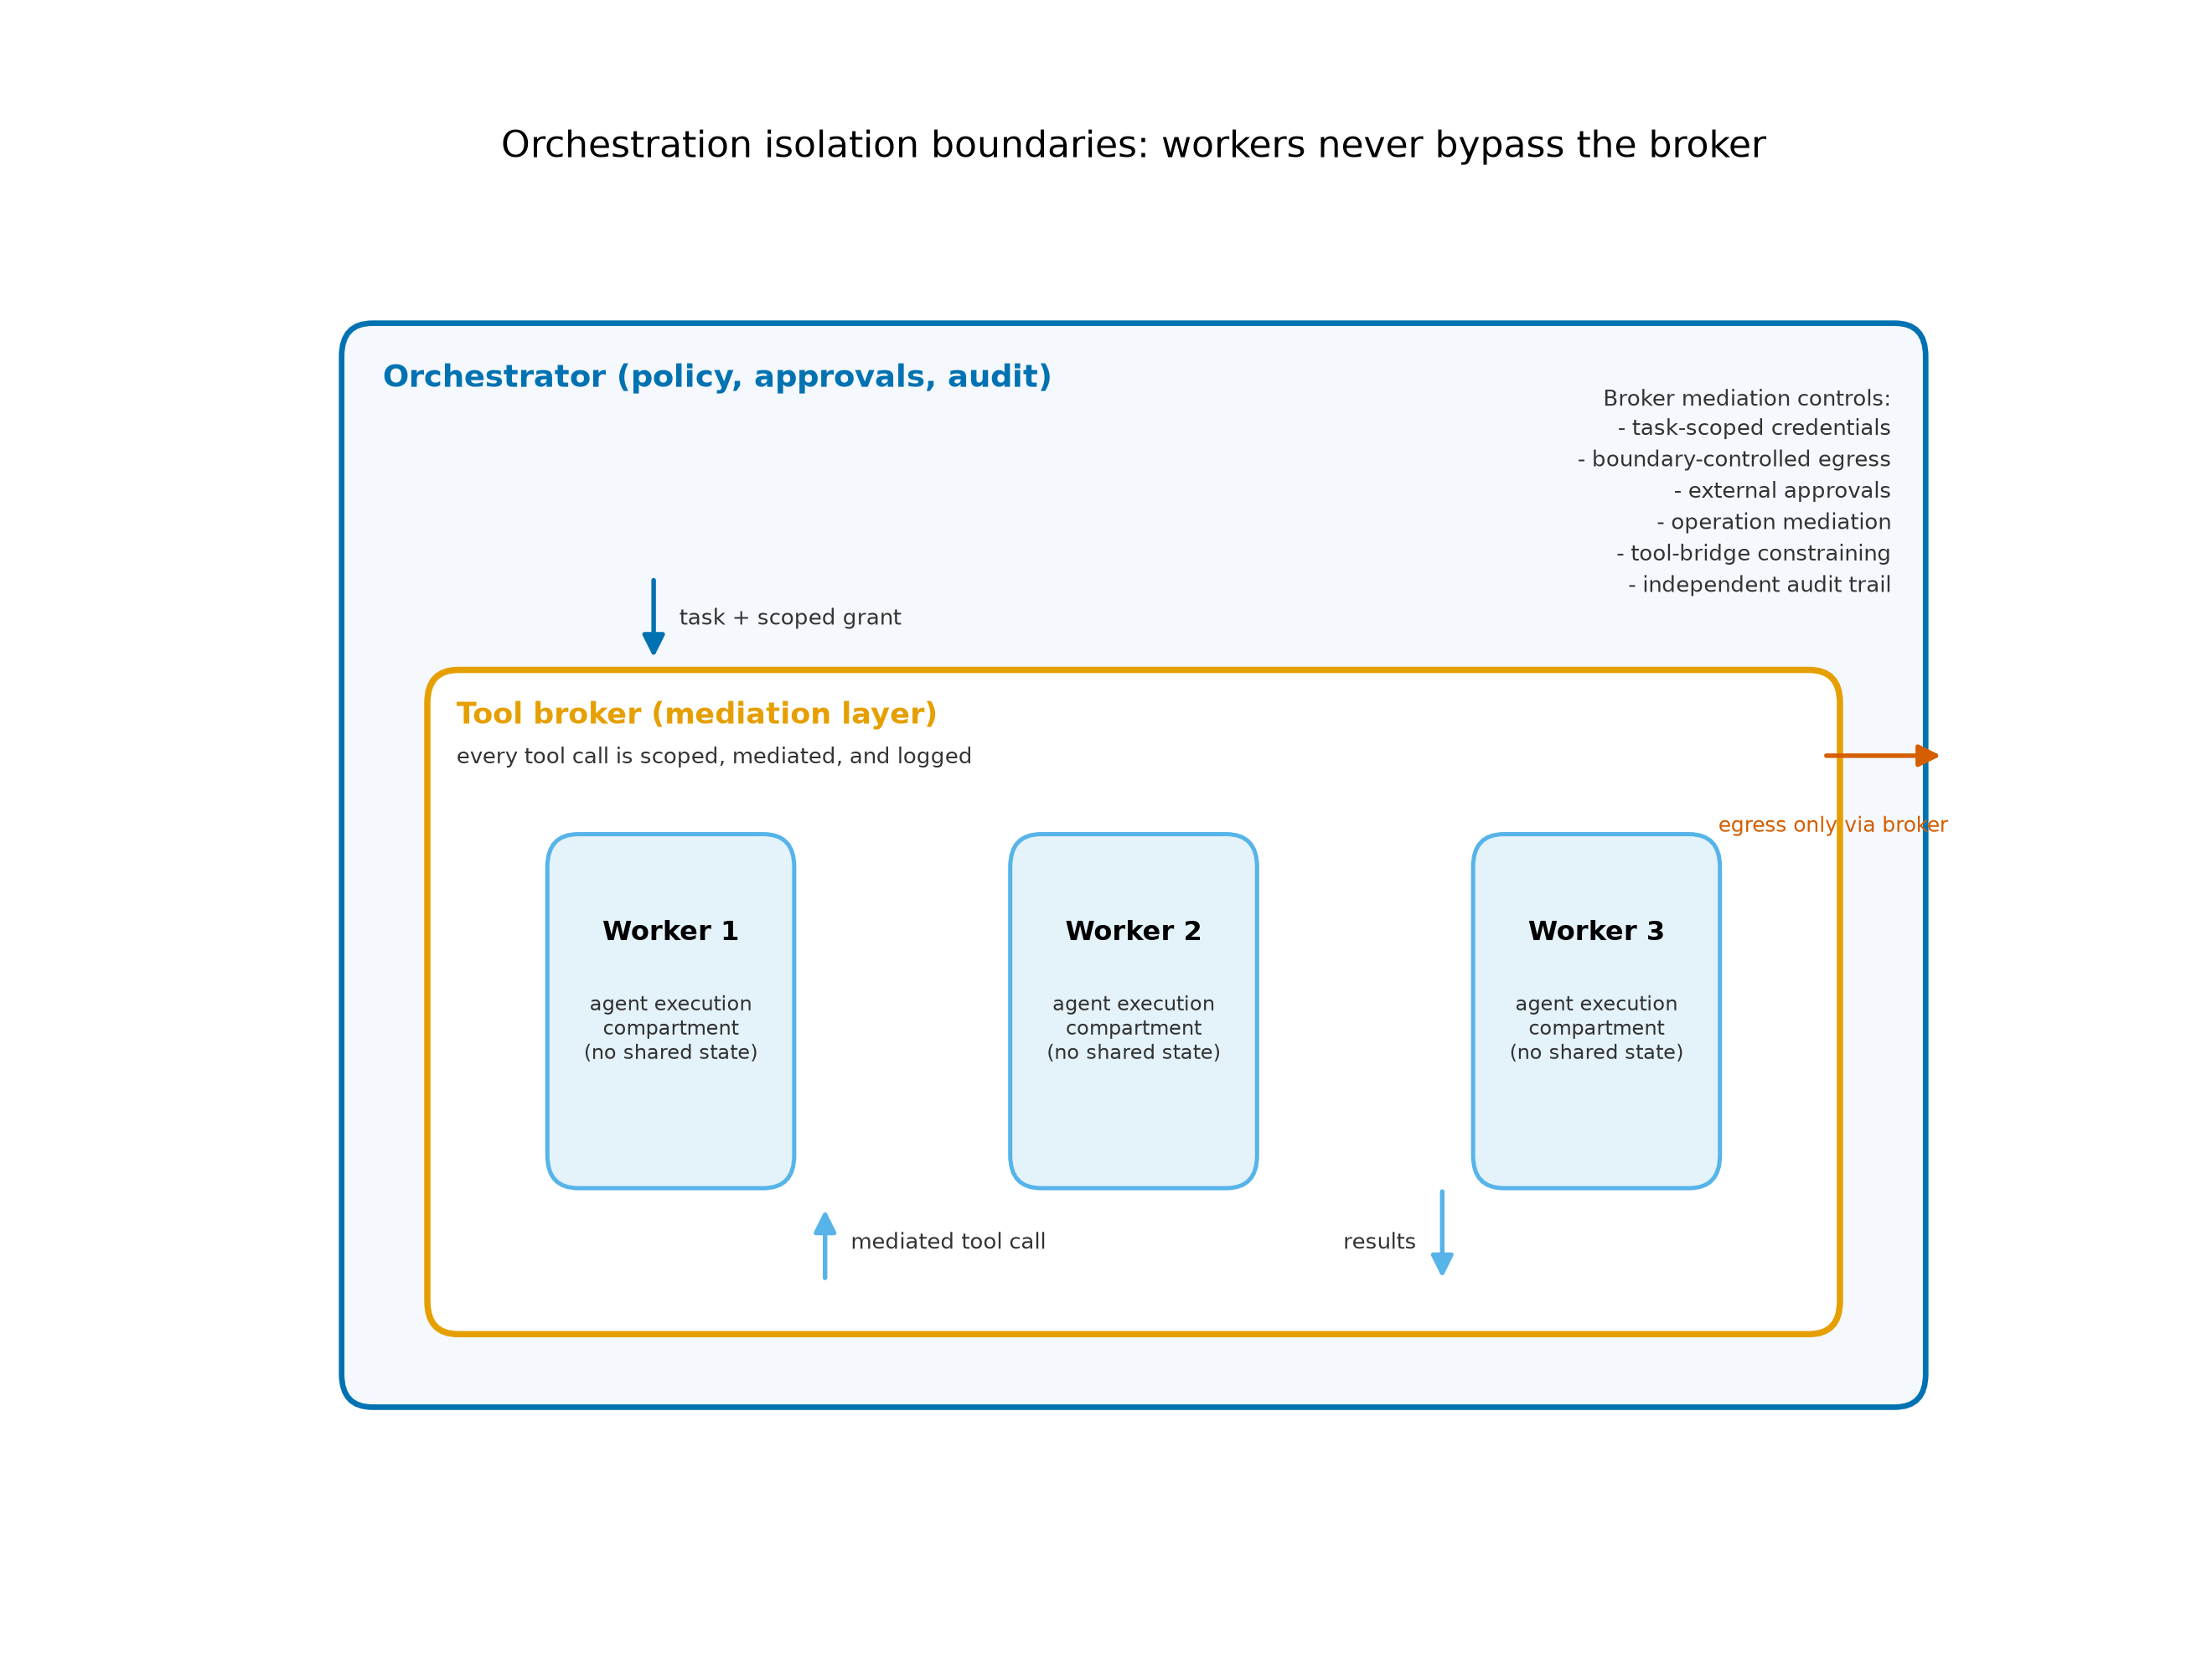
\includegraphics[width=1\linewidth,height=0.40\textheight,keepaspectratio,alt={A reference orchestration: one orchestrator delegating through an MCP-style tool broker to three disposable workers, with the ten mediation points numbered at each trust-boundary crossing.}]{../figures/orchestration_boundaries.png}
\caption{A reference orchestration: one orchestrator delegating through
an MCP-style tool broker to three disposable workers, with the ten
mediation points numbered at each trust-boundary
crossing.}\label{fig:orchestration_boundaries}
\end{figure}

\end{frame}

\begin{frame}[fragile,allowframebreaks]{Delegation chains and the
confused deputy}
The boundaries in fig.~\ref{fig:orchestration_boundaries} are the
orchestration-layer rendering of the trust-domain design: executors
instantiate the \texttt{agent\_execution} domain, broker policy carries
the \breaktt{credential\_service} restrictions, external approval
embodies the \texttt{administration} and \breaktt{release\_deployment}
requirements, and the audit trail belongs to the recovery domain of
tbl.~8.
\end{frame}

\begin{frame}[allowframebreaks]{The mediation-point taxonomy}
\protect\phantomsection\label{the-mediation-point-taxonomy}
The mechanisms reviewed in this section reduce to ten mediation points:
places where an orchestration stack can interpose a check between an
agent capability and an agent action. Each is already instantiated in
deployed systems rather than proposed for the future.

\end{frame}

\begin{frame}[allowframebreaks]{The mediation-point taxonomy}
\begin{enumerate}
\tightlist
\item
  \textbf{Sandbox primitives} --- the process/host boundary: bubblewrap,
  Seatbelt, and Landlock restrict filesystem, process, and namespace
  reach before any tool call happens (Anthropic 2026b; OpenAI 2026; L.
  K. Project 2026).
\item
  \textbf{Egress proxy} --- the agent/network boundary: outbound traffic
  passes a proxy whose allowlist, not the agent's request text, decides
  the destination (Anthropic 2026b).
\item
  \textbf{Tool annotations} --- advisory capability metadata on MCP
  tools; useful for surfacing risk to humans, explicitly not a guarantee
  (Project 2025c).
\item
  \textbf{OAuth resource-server binding} --- protected-resource metadata
  per RFC 9728 and audience-bound tokens per RFC 8707, so a credential
  presented anywhere else fails (Project 2025d).
\item
  \textbf{URL-mode elicitation} --- browser-based authorization in which
  the client never handles user credentials (Project 2025a).
\item
  \textbf{Agent-to-agent transport security} --- A2A's mandatory TLS and
  standard HTTP authentication between opaque agents (Foundation 2026).
\item
  \textbf{Agent identity exchange} --- SPIFFE/WIMSE workload identity
  with RFC 8693 token exchange and transaction tokens for short-lived,
  downscoped delegation (Force 2026).
\item
  \textbf{Classifier escalation} --- actions an automated classifier
  flags as resembling misuse are routed through two-stage review, as in
  Anthropic's auto-mode containment design (Anthropic 2026a).
\item
  \textbf{Sandbox observability} --- audit instrumentation at the
  sandbox boundary, such as gVisor's SecCheck, recording what the agent
  attempted independently of what it reports (gVisor Project 2026).
\item
  \textbf{External approval} --- the human or deterministic-policy gate
  for consequential actions, outside the proposing hierarchy
  (tbl.~9).
\end{enumerate}

\end{frame}

\begin{frame}[allowframebreaks]{The mediation-point taxonomy}
Mapped against the agent capability classes of
sec.~10 --- content intake, tool and bridge
use, credential touch, external communication, state mutation,
self-modification --- the taxonomy shows where mechanical coverage
exists. External communication crosses points 2, 4, and 6; credential
touch crosses 4, 5, and 7; state mutation and self-modification are
contained by 1 and audited by 9; tool and bridge use is broker-mediated
under policy informed by 3. Content intake has no mechanical point at
all --- hostile content enters through any permitted channel --- which
is why the cognitive-security analysis of
sec.~11 and the external-approval point 10
carry the weight mediation cannot. The coding-agent platforms'
convergence on points 1, 2, and 8 --- OS-primitive sandboxing, proxy
egress, classifier escalation (Anthropic 2026b; OpenAI 2026; Google
2026) --- before the protocol work standardizes points 4 through 7, is
\end{frame}

\begin{frame}[allowframebreaks]{The mediation-point taxonomy}
the market's own vote on where control belongs.
fig.~\ref{fig:agent_surface} arranges the matrix, with the numbered
mediation points keyed to the list above.

\end{frame}

\begin{frame}[allowframebreaks]{The mediation-point taxonomy}
\begin{figure}
\centering
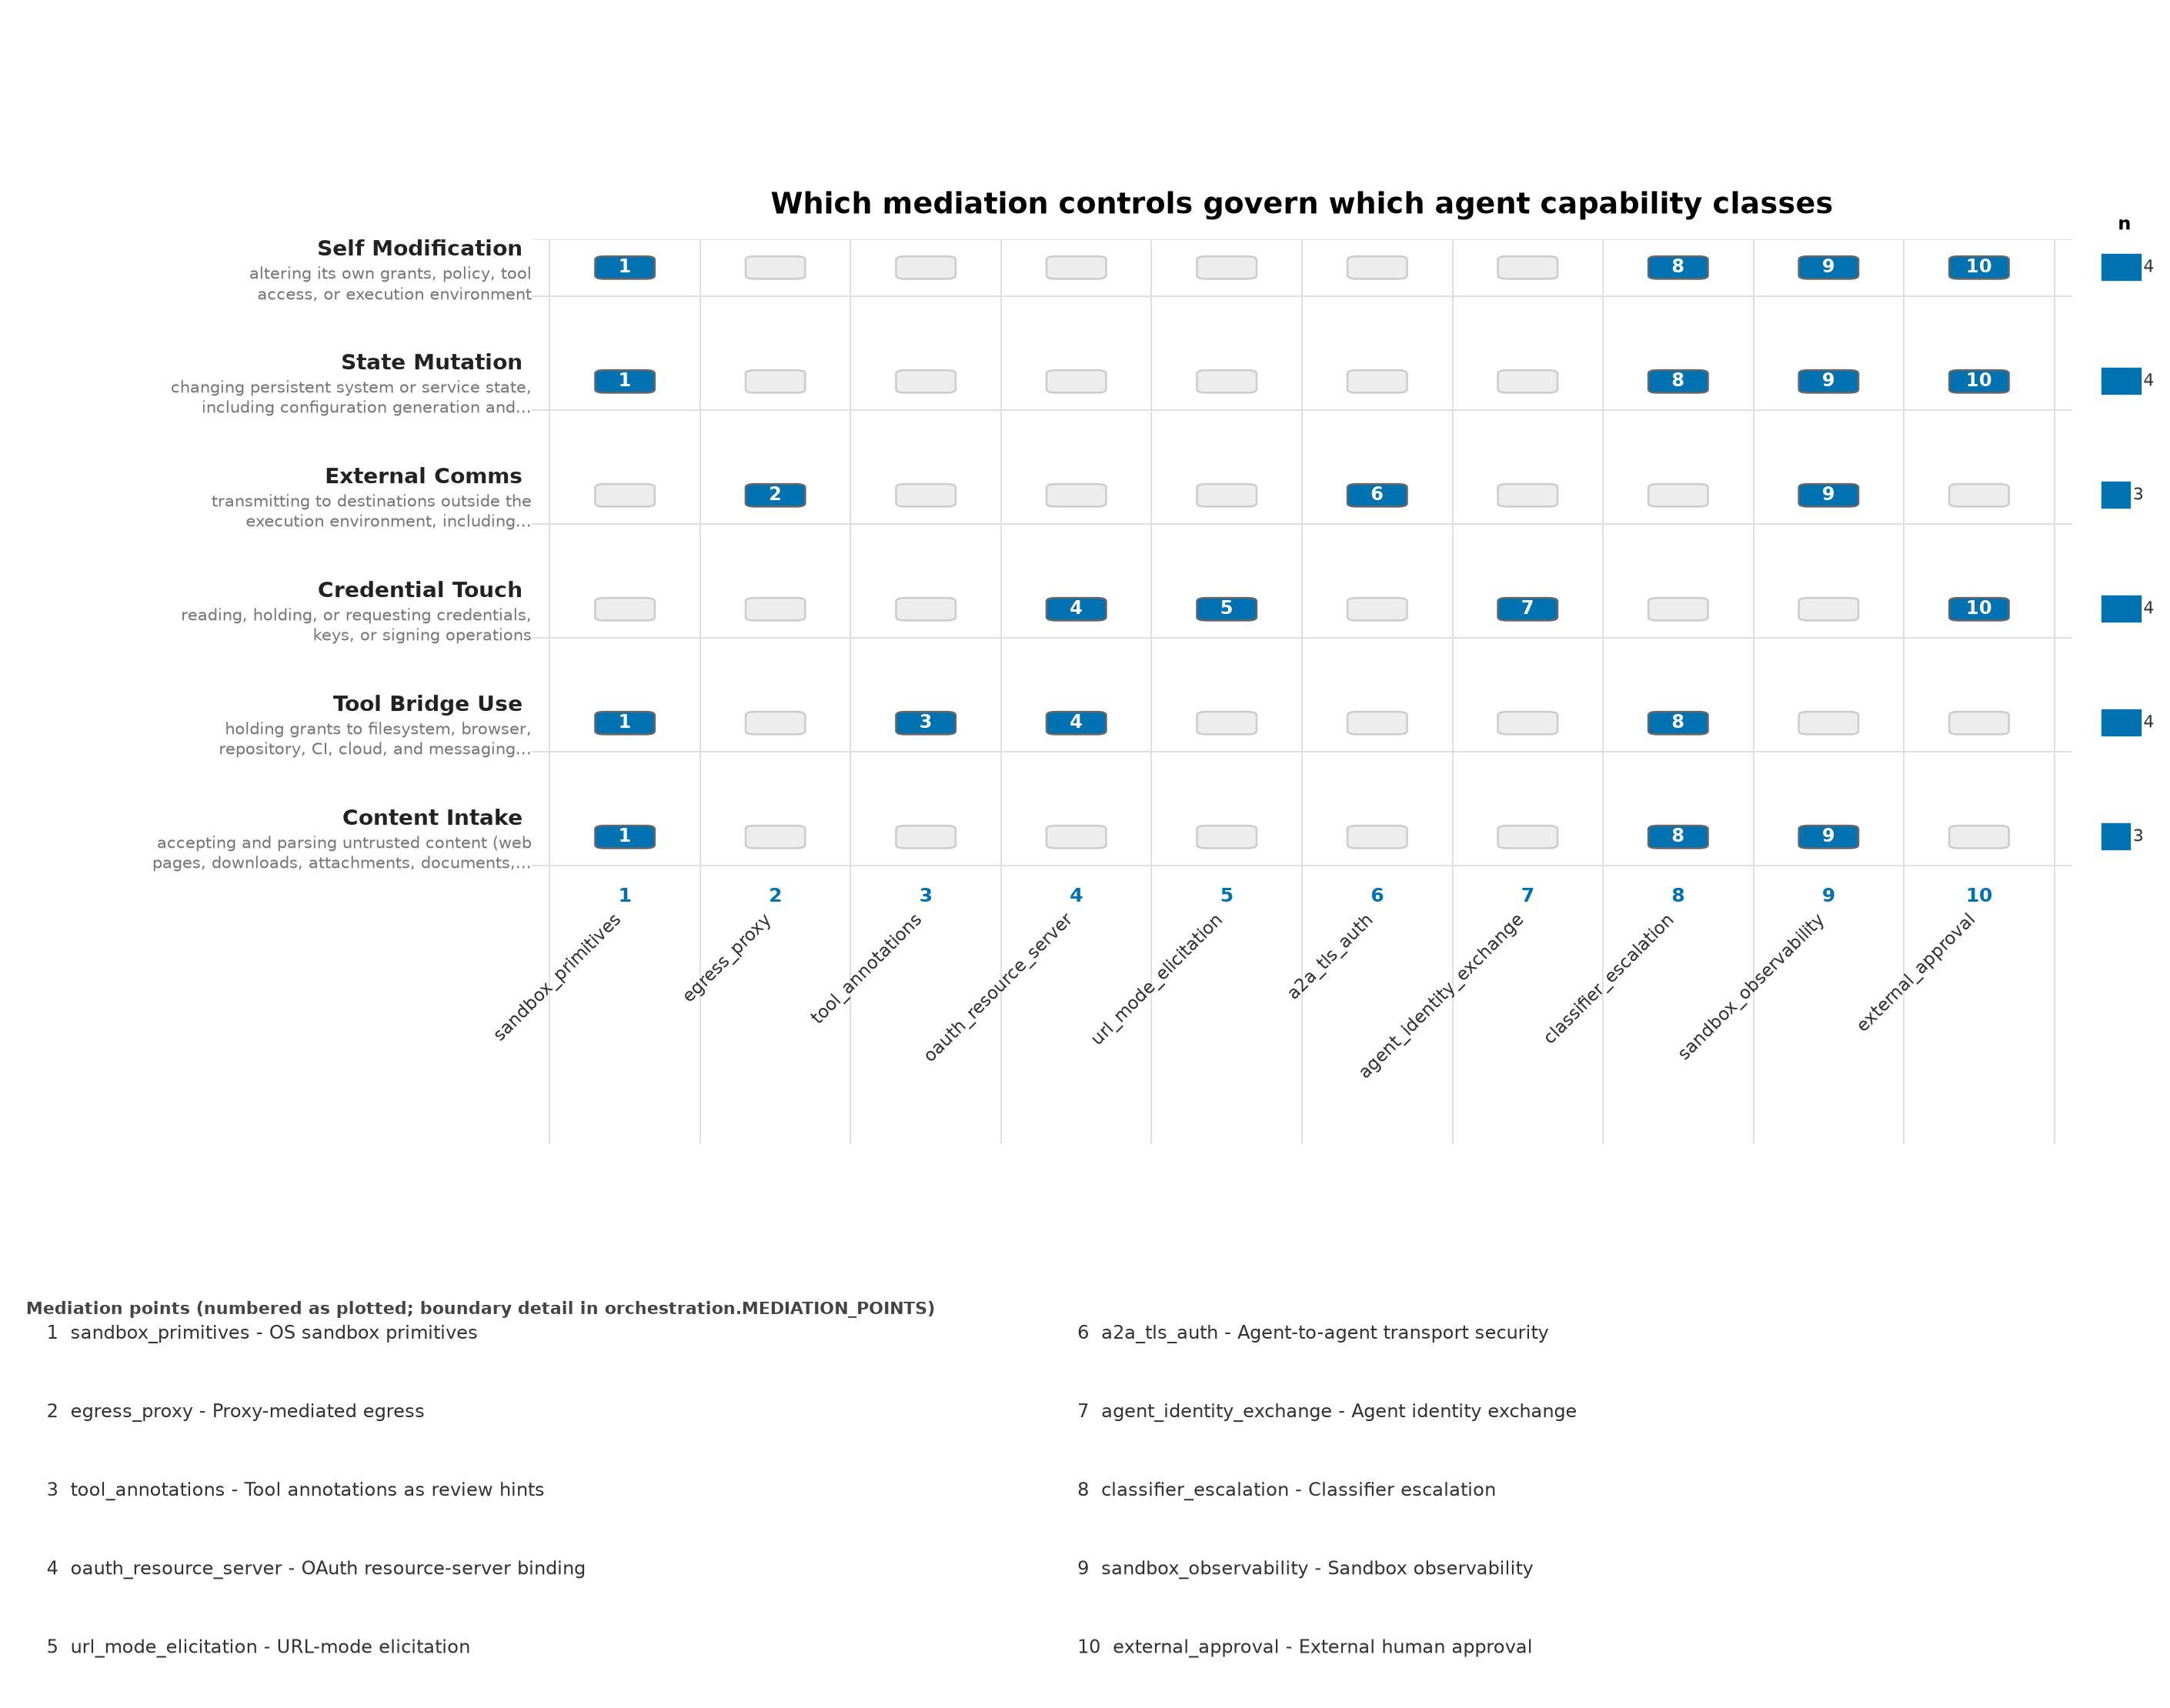
\includegraphics[width=1\linewidth,height=0.40\textheight,keepaspectratio,alt={Which mediation point constrains which agent capability class; filled numbered cells mark the primary control, and the right marginal counts how many distinct controls cover each capability.}]{../figures/agent_surface.png}
\caption{Which mediation point constrains which agent capability class;
filled numbered cells mark the primary control, and the right marginal
counts how many distinct controls cover each
capability.}\label{fig:agent_surface}
\end{figure}
\end{frame}

\begin{frame}[allowframebreaks]{Approval chains across agent
hierarchies}
\protect\phantomsection\label{approval-chains-across-agent-hierarchies}
The configuration invariant that no component may approve its own policy
changes (sec.~14) applies with full
force here: an orchestrator that can propose a consequential operation
and also approve it has collapsed the separation between proposal and
authorization that the authority ladder of
sec.~10 maintains across its rungs. Approval
must originate outside the hierarchy --- a human principal, or a
deterministic policy check with no stake in the task's completion. A
second AI instance reading the same hostile material is not an
independent approval boundary: it shares the attacker's channel into the
first agent's context (sec.~11). Approval
context should carry the operation's full parameters --- artifact,
destination, scope, expiration --- so the approver decides about the
actual operation rather than about a summary of it; and the approval
\end{frame}

\begin{frame}[allowframebreaks]{Approval chains across agent
hierarchies}
path itself, like the transfer paths of sec.~5, is a
high-value component whose compromise routes around every other control.
\end{frame}

\begin{frame}[allowframebreaks]{Auditability of multi-agent decisions}
\protect\phantomsection\label{auditability-of-multi-agent-decisions}
Multi-agent decisions are hard to reconstruct because intent is
distributed: no single transcript contains why a task evolved as it did,
and agent prose is a poor record of authority events. The audit
obligation (tbl.~9, independent audit) therefore
attaches to the structure. Record every tool-broker decision with its
full request context; record every credential mint, use, and revocation;
record every delegation edge --- which planner asked which worker for
what, with which inputs and which returned artifacts. The record lives
outside every agent's write authority and outside the orchestrator's,
because rewriting the audit trail is one of the 9 configuration
invariants of sec.~14.
Sandbox-boundary observability is the enforcement instrument for the
agent-side half of this obligation: an instrumentation point such as
gVisor's SecCheck records system-level behavior at the sandbox edge,
\end{frame}

\begin{frame}[allowframebreaks]{Auditability of multi-agent decisions}
which is the record an operator can compare against what the agent
narrated (gVisor Project 2026). Make the record useful for
reconstructing what happened: timestamps, operation parameters, policy
verdicts, and approver identities, not collected narration.
\end{frame}

\begin{frame}[fragile,allowframebreaks]{Mapping to the trust-domain
architecture}
\protect\phantomsection\label{mapping-to-the-trust-domain-architecture}
The mapping closes the loop with sec.~10. The
orchestrator's decomposition and aggregation role sits adjacent to
\texttt{administration}, with no standing production credentials of its
own. Executors instantiate \texttt{agent\_execution} under its
restrictions: no host home, no broad credential directory, no ambient
production session. The broker instantiates the
\breaktt{credential\_service} discipline: it exposes specific operations,
not raw secrets or shells. Result intake applies the
\texttt{browsing\_intake} restrictions: aggregated worker output is
untrusted material, reviewed before promotion. Deployment endpoints
apply the \breaktt{release\_deployment} rule: agents may propose, but
external approval must be unalterable by any of the proposing parties.
The audit trail and known-good configuration instantiate
\texttt{recovery}, beyond the destructive authority of everything above
\end{frame}

\begin{frame}[fragile,allowframebreaks]{Mapping to the trust-domain
architecture}
them. Orchestration does not replace this architecture; it is the layer
where the architecture's rules are either enforced by construction or
quietly dissolved by convenience.
\end{frame}

\end{document}
